\chapter{Método Proposto}
\label{sec:method}
Este capítulo descreve a metodologia desenvolvida para a classificação automática dos graus ISUP em imagens histológicas de biópsias de próstata. A Figura \ref{fig:propostatese} apresenta uma visão do fluxo de trabalho implementado, que é subdividido em quatro etapas fundamentais, a serem exploradas sequencialmente neste capítulo. Inicialmente, a Seção \ref{sec:method_materiais} descreve os materiais utilizados, com foco nas características do \textit{dataset} PANDA. Em seguida, a Seção \ref{sec:pre} detalha o pré-processamento, abordando as estratégias de divisão de dados, a análise de entropia para filtragem de amostras ruidosas e a extração de \textit{patches}. A terceira etapa, descrita na Seção \ref{sec:train_models}, engloba o Treinamento e Modelos, nos quais são discutidos a otimização de hiperparâmetros e o treinamento dos modelos EfficientNet (B0, B3 e B7) sob diferentes configurações de funções de perda ordinais. Por fim, a Seção \ref{sec:ensemble} apresenta a Avaliação do \textit{Ensemble}, elucidando as estratégias de fusão de modelos (Média, Máximo e Voto) adotadas para consolidar a predição final do grau ISUP.

\label{cap:materiais-metodo}
\begin{figure}[H]
	\caption{Etapas do Método Proposto}
	\centering
	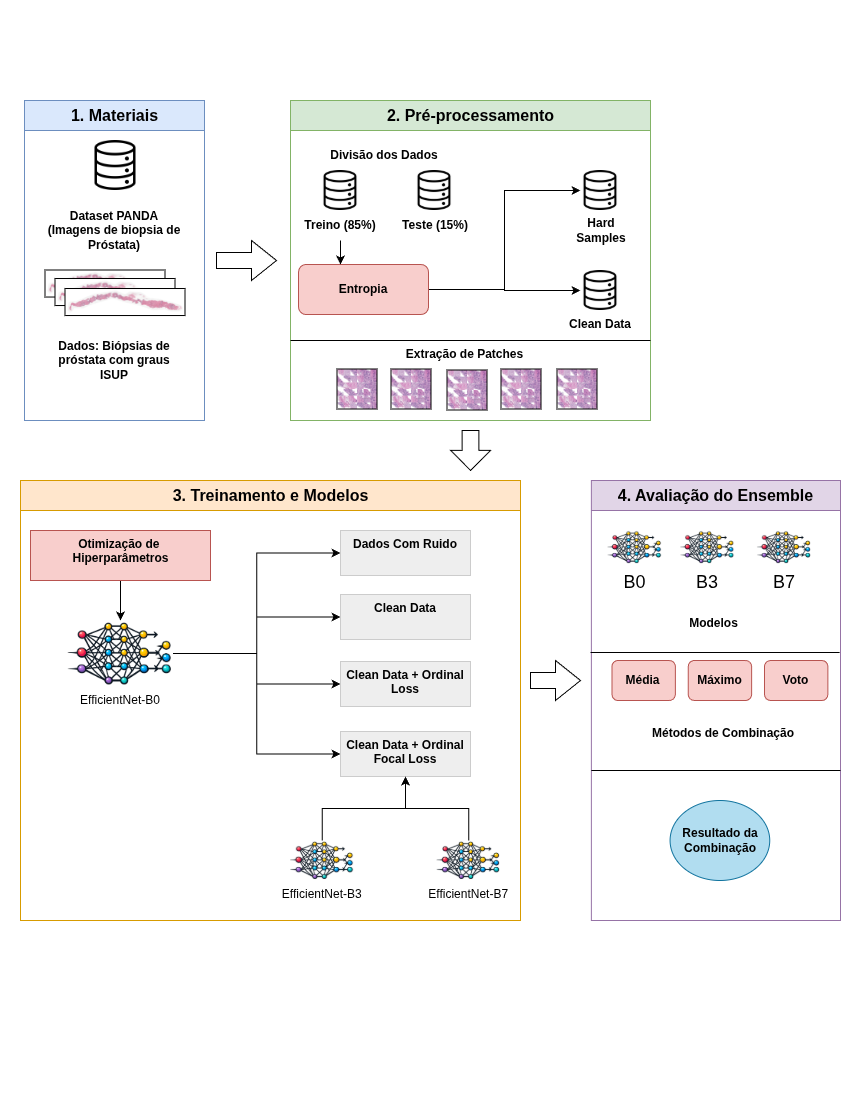
\includegraphics[width=1\linewidth]{figuras/proposta_tese}
	
	\label{fig:propostatese}
\end{figure}

\section{Materiais}
\label{sec:method_materiais}

Neste trabalho, utilizou-se o conjunto de dados PANDA (\textit{Prostate Cancer Grade Assessment}), composto por aproximadamente 10.616 imagens histopatológicas completas de biópsias de próstata \cite{ref-panda2020}.
Este conjunto de dados foi disponibilizado como parte do desafio PANDA na plataforma Kaggle e tem sido amplamente utilizado em pesquisas sobre a classificação automática do câncer de próstata.
As imagens no conjunto de dados são anotadas com o escore e o grau de Gleason, fornecendo rótulos clínicos utilizados na graduação da doença.
Neste estudo, apenas a versão pública do conjunto de dados foi utilizada, sem acesso ao conjunto de teste privado disponibilizado no desafio. Os dados foram coletados em dois centros médicos, \textit{Radboud University Medical Center} e \textit{Karolinska Institute}, o que introduz variabilidade institucional nas imagens.

Essa variabilidade está associada a diferenças nos protocolos de preparação de lâminas, nos procedimentos de escaneamento e nos critérios de anotação, o que aproxima o cenário experimental da prática clínica.
Além disso, o conjunto de dados apresenta ruídos inerentes tanto ao processo de aquisição quanto ao de anotação das lâminas. Entre os artefatos visuais, destacam-se marcas de caneta realizadas por patologistas durante a análise, como ilustrado na Figura~\ref{fig:pen_mask}, que podem interferir na extração de características relevantes pelos modelos. Adicionalmente, há fontes de ruído associadas à rotulagem, incluindo a variabilidade interobservador na atribuição dos graus histopatológicos, o que introduz incerteza nos rótulos de treinamento. Nesse contexto, \cite{kabir2025automating} relatam inconsistências entre diferentes níveis de anotação, evidenciando casos em que as máscaras de segmentação não estavam alinhadas aos rótulos globais das respectivas imagens. Tais discrepâncias comprometem a qualidade supervisionada dos dados e podem prejudicar o processo de aprendizado, especialmente em tarefas que dependem da coerência entre anotações locais e globais.

Esses fatores aumentam a complexidade da tarefa de classificação automática e refletem desafios presentes na prática da patologia digital.

\begin{figure}[H]
	\centering
	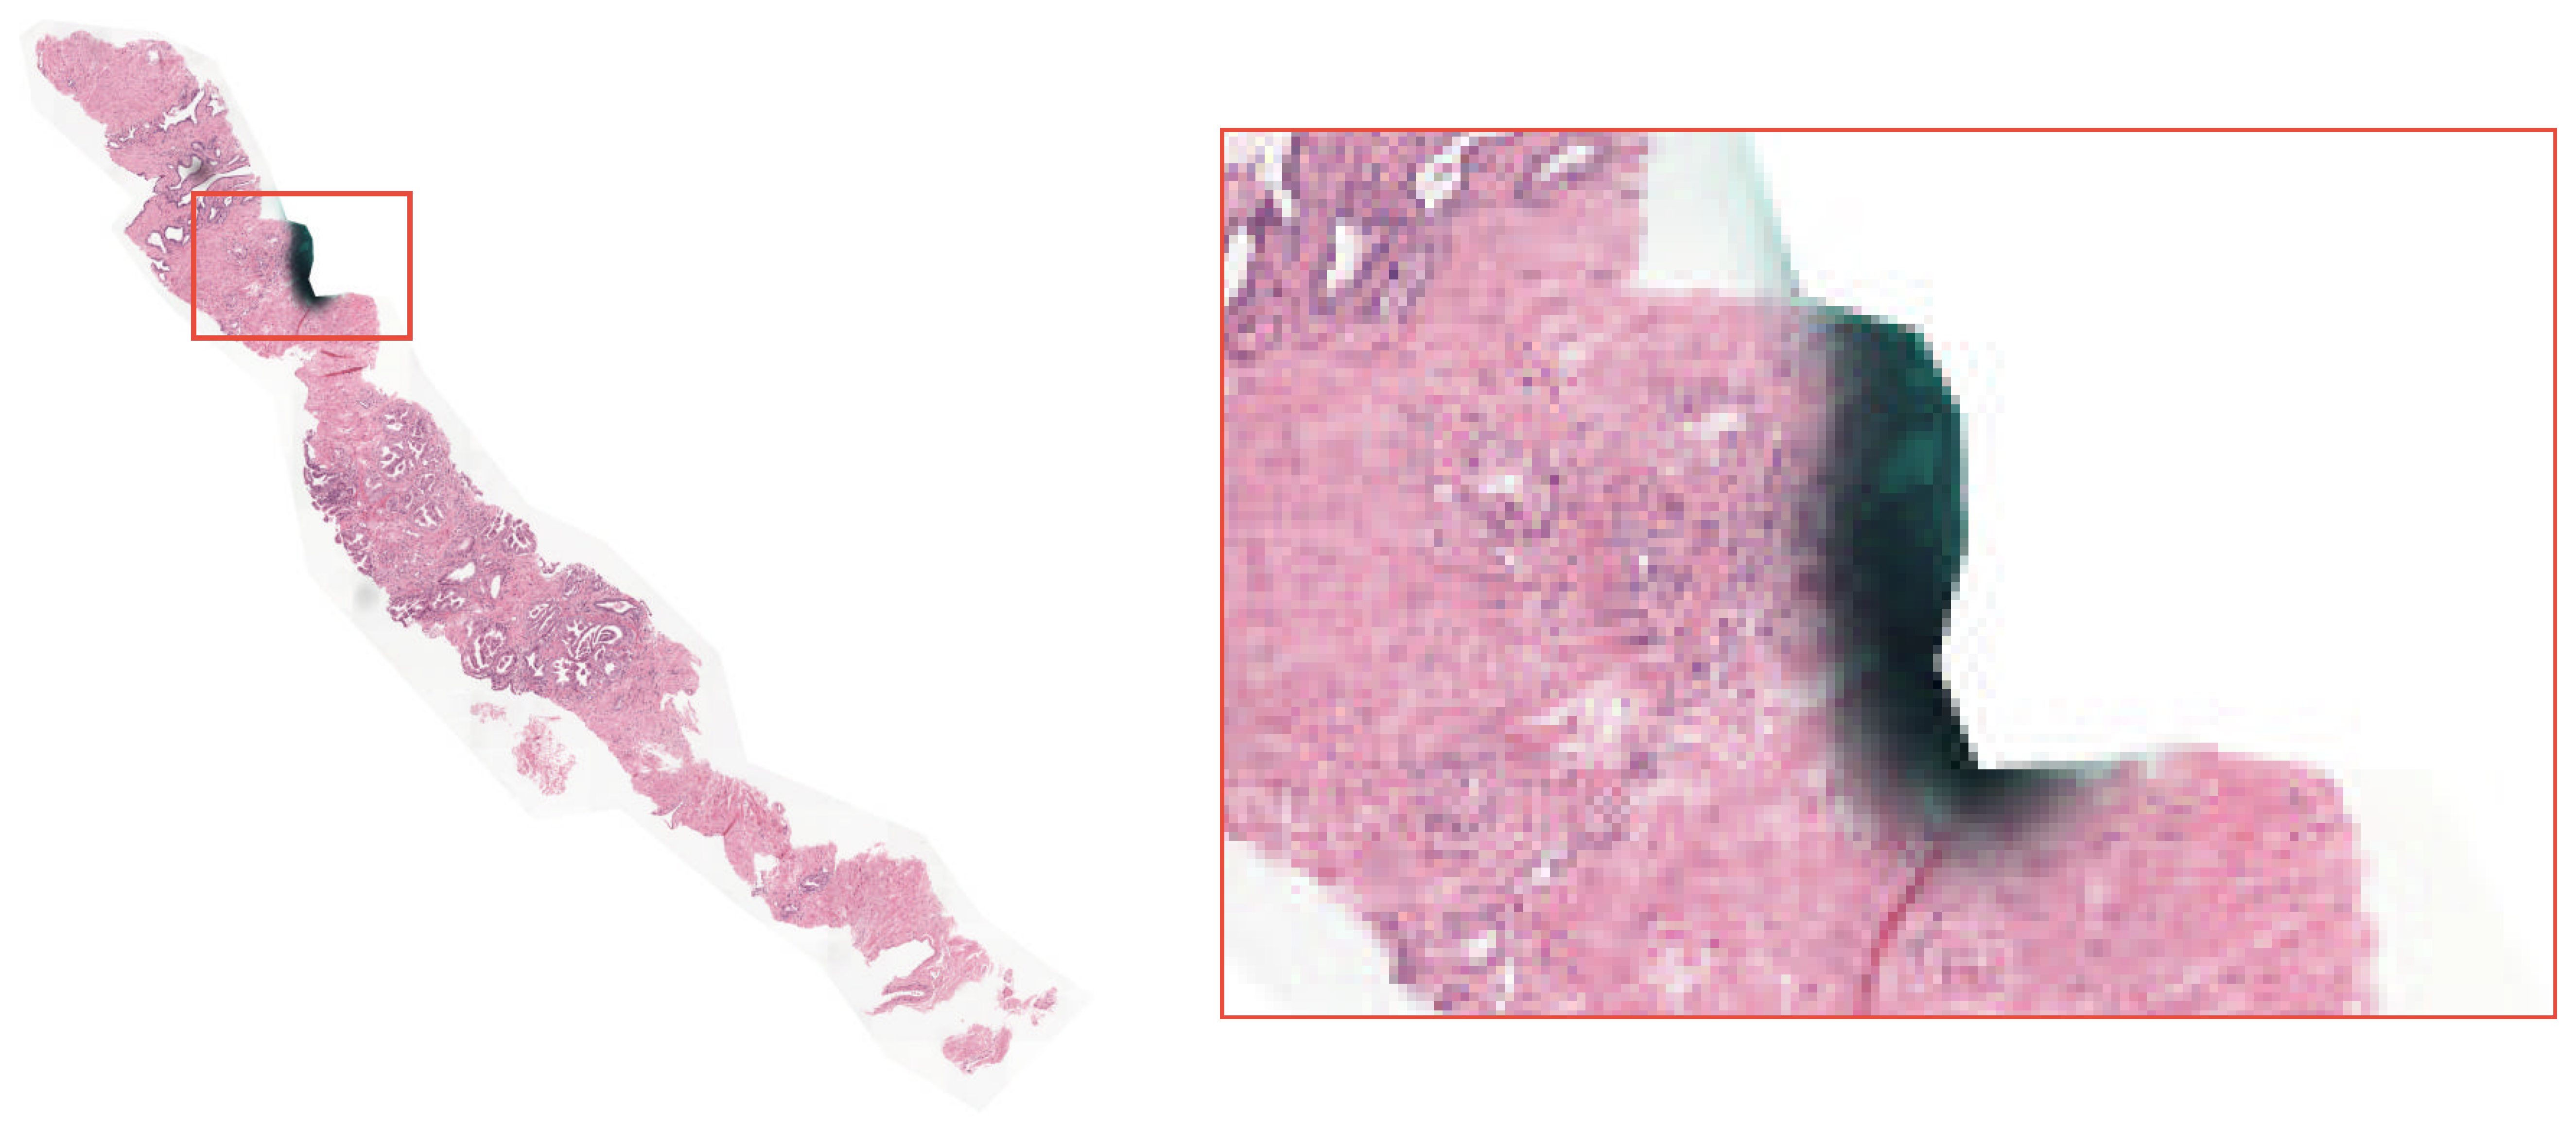
\includegraphics[width=0.8\linewidth]{figuras/zoom_region.png}
	\caption{Exemplo de um artefato visual presente em uma WSI do conjunto de dados PANDA.
		À esquerda, apresenta-se a lâmina completa, com a região de interesse destacada em vermelho.
		À direita, uma visão ampliada da região selecionada revela uma marca de caneta sobre o tecido prostático. \\
		Fonte: Elaborado pelo autor.
	}
	\label{fig:pen_mask}
\end{figure}

Outro aspecto relevante do conjunto de dados é a distribuição desigual das amostras entre as seis classes de graduação (ISUP 0 a ISUP 5). Esse desbalanceamento torna-se evidente na Figura \ref{fig:distribuicao-isup}, que apresenta a distribuição das amostras por classe. Observa-se que a maior parte dos exemplos está concentrada nas classes ISUP 0 e ISUP 1.

\begin{figure}[H]
	\centering
	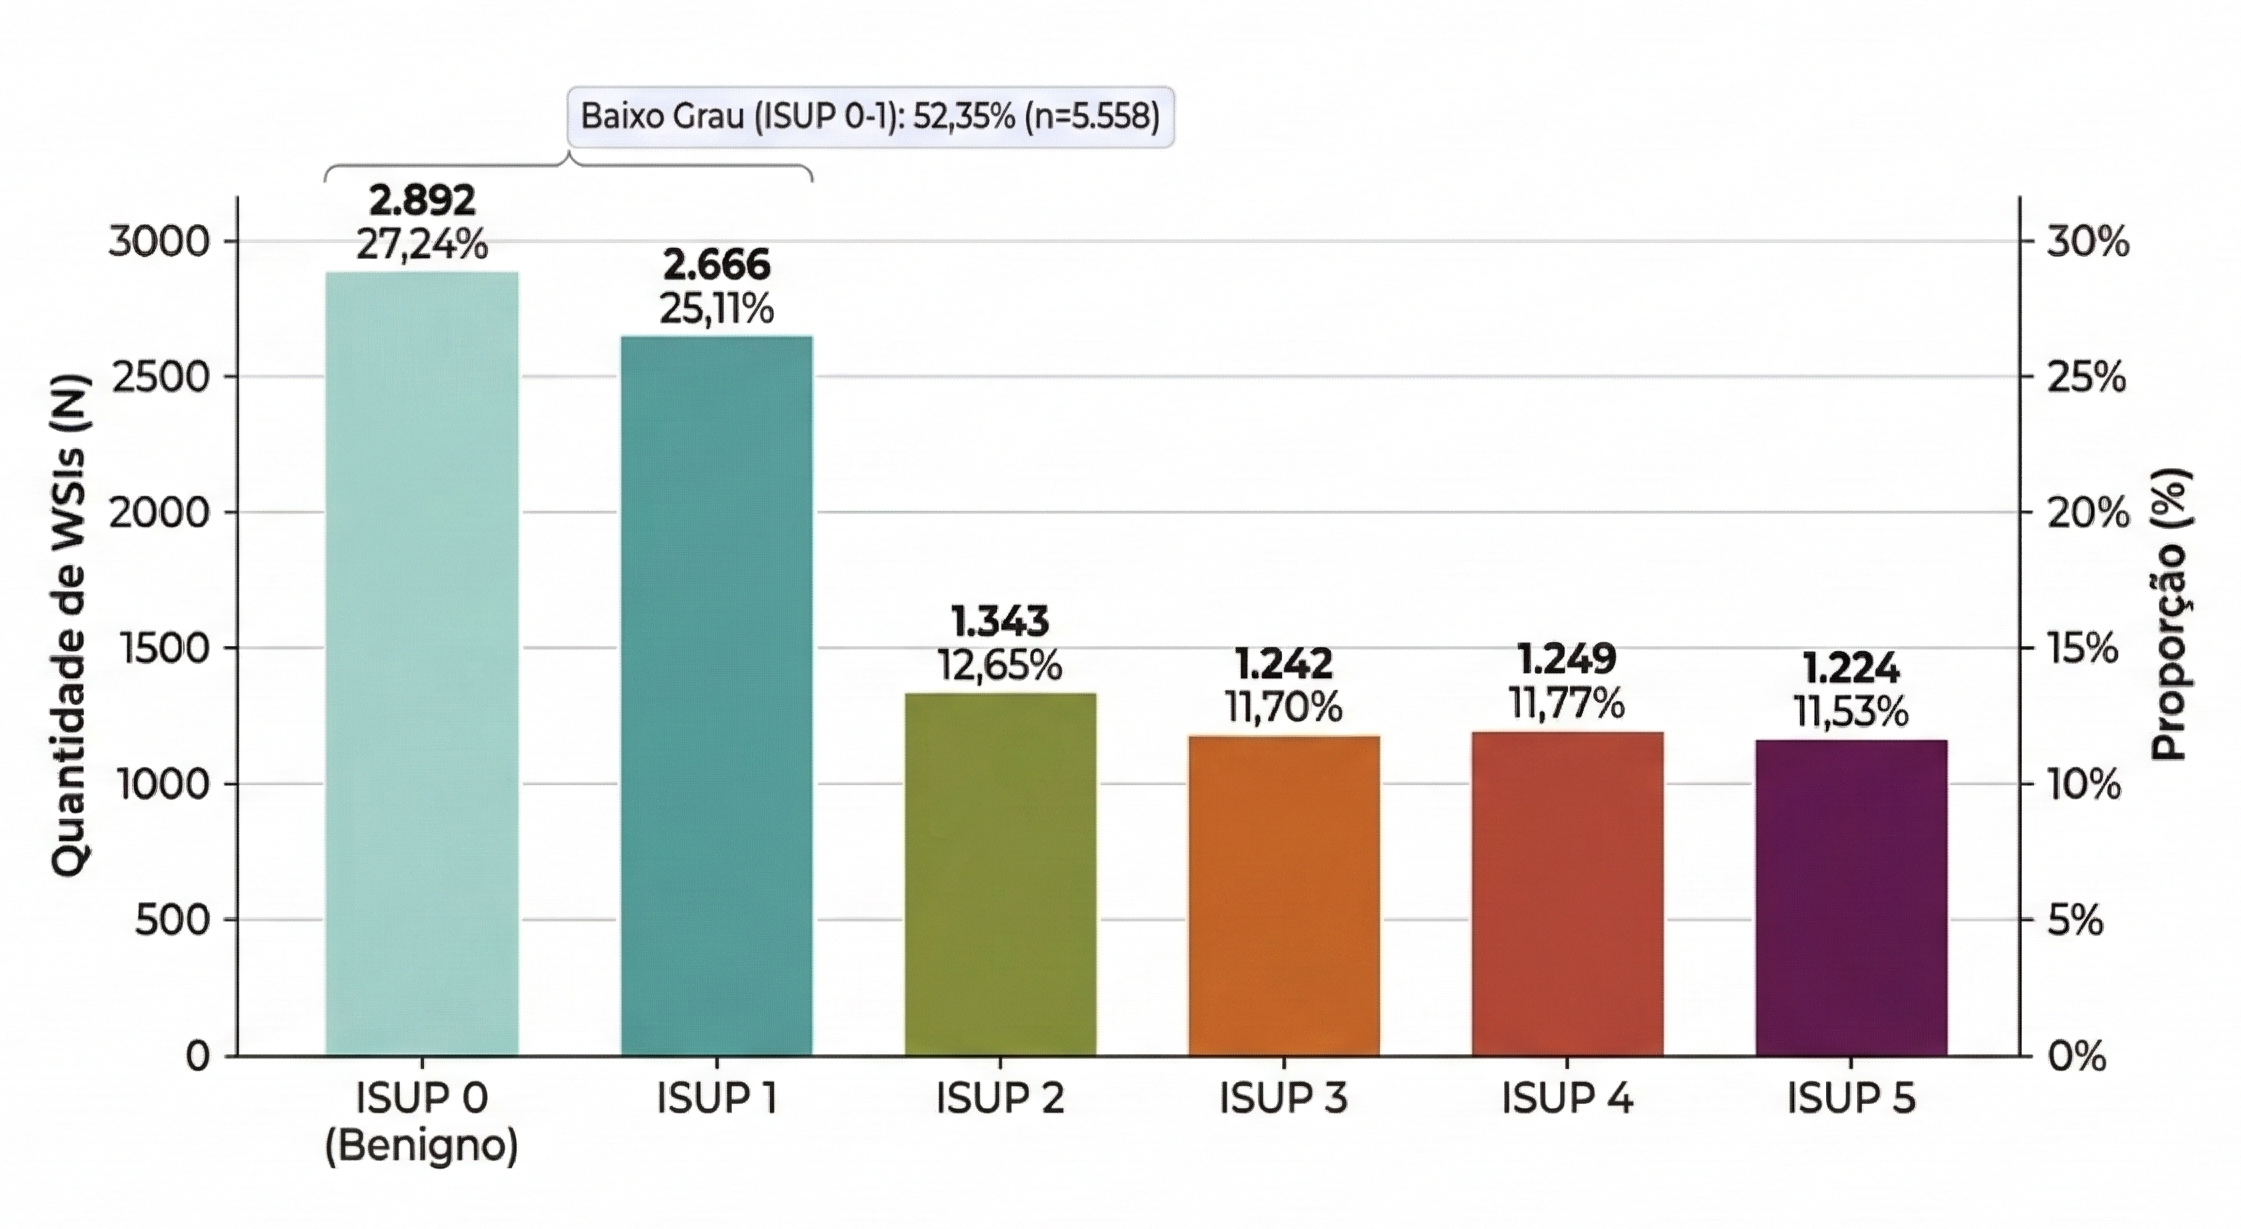
\includegraphics[width=1\textwidth,height=0.3\textheight]{figuras/distribuicao_ISUP.png}
	\caption{Distribuição de amostras no conjunto de dados PANDA}
	\label{fig:distribuicao-isup}	
\end{figure}

\section{Pré-processamento}
\label{sec:pre}

O fluxo de pré-processamento foi estruturado em duas etapas sequenciais: a filtragem de ruído nos rótulos e a extração de \textit{patches}. Inicialmente, o conjunto de dados foi dividido em treinamento (85\%) e teste (15\%), garantindo independência entre o processo de ajuste e a avaliação final dos modelos. Após essa divisão, o conjunto de treinamento passou a conter 9.024 instâncias, enquanto o conjunto de teste, utilizado na avaliação de todos os modelos deste trabalho, ficou composto por 1.592 instâncias.


\subsection{Filtragem de Ruído Baseada em Entropia}
\label{sub:entropia}

Conforme relatado na Seção~\ref{sec:method_materiais}, o conjunto PANDA apresenta ruídos nos rótulos, decorrentes de anotações manuais e de laudos patológicos inconclusivos. Para mitigar o impacto dessas inconsistências no aprendizado, foi aplicada uma estratégia de filtragem baseada na estimativa de incerteza preditiva.

Inicialmente, considerou-se o conjunto de treinamento correspondente a 85\% das amostras do \textit{dataset} completo. Esse conjunto foi subdividido em duas partes: 80\% das amostras foram utilizadas para treinamento efetivo dos modelos, enquanto os 20\% restantes foram reservados para validação interna. Em seguida, quatro variantes de menor complexidade da família EfficientNet (B0, B1, B2 e B3) foram treinadas de forma independente utilizando essa divisão. Cada modelo foi treinado por 20 épocas, com taxa de aprendizado inicial de $3 \times 10^{-4}$, critério de parada antecipada (\textit{early stopping}) com paciência de 7 épocas, e função de perda baseada em \textit{Binary Cross-Entropy} (BCE).

Após o treinamento, cada modelo foi utilizado para gerar probabilidades preditas para todas as amostras dos conjuntos de treinamento e validação. Essas predições foram posteriormente empregadas para estimar a incerteza e identificar amostras potencialmente ruidosas.
A incerteza de cada decisão foi quantificada usando a entropia de Shannon \cite{ali2023entropy}, definida para a classe $c$ como:

\begin{equation}
	H = \frac{1}{C} \sum_{c=1}^{C} -\big[p_c \log(p_c) + (1-p_c)\log(1-p_c)\big],
\end{equation}

Onde $p_c$ é a probabilidade predita para a classe positiva e $C$ é o número de classes. Valores de $p_c$ próximos de 0 ou 1 indicam baixa entropia (alta confiança), enquanto valores próximos de 0.5 refletem alta incerteza.  

A entropia foi calculada para cada amostra em cada modelo e, em seguida, foi obtida a média das predições das quatro redes. Com base nessa estimativa, foram selecionadas as 10\% amostras com maior entropia média, calculadas exclusivamente sobre o conjunto de treinamento, ou seja, correspondentes a 10\% das amostras pertencentes a esse conjunto (85\% do dataset total), formando um subconjunto denominado \textit{hard samples}.

A partir desse conjunto, avaliou-se o impacto da remoção dessas amostras apenas no conjunto de treinamento, considerando quatro cenários experimentais:

\begin{itemize}
	\item (i) utilização de todo o conjunto de dados (sem remoção de \textit{hard samples});
	\item (ii) remoção de 100\% das \textit{hard samples};
	\item (iii) remoção de 50\% das \textit{hard samples};
	\item (iv) remoção de 20\% das \textit{hard samples}.
\end{itemize}

\subsection{Extração de Patches}
\label{sub:patches}

Após a definição das amostras de treinamento por meio da filtragem de entropia, a etapa final do pré-processamento consistiu na geração das imagens de entrada para o modelo final. Como o tecido histológico ocupa apenas uma fração da WSI, como observamos na Figura~\ref{fig:original-panda}, processar a lâmina completa exigiria um custo computacional elevado e seria desnecessário para tratar extensas áreas de fundo.

\begin{figure}[H]
	\centering
	
\includegraphics[width=0.8\linewidth]{figuras/original.png}
	\caption{Imagem de exemplo do conjunto de dados PANDA evidenciando a vasta área sem tecido.}
	\label{fig:original-panda}
\end{figure}

Para extrair regiões informativas das imagens, adotou-se uma abordagem baseada na geração de recortes (\textit{patches}) da imagem original. Inicialmente, definiu-se um tamanho fixo de $256 \times 256$ \textit{pixels} para cada \textit{patch}. Para garantir a padronização, aplicou-se preenchimento com \textit{pixels} brancos nas bordas das WSIs, de modo que suas dimensões se tornassem compatíveis com a extração de \textit{patches} de tamanho fixo. Em seguida, cada imagem foi particionada em \textit{patches}, e a presença de tecido em cada fragmento foi estimada pela soma dos valores RGB; como o fundo tende ao branco, menores somas indicam maior densidade de tecido. Os \textit{patches} foram então ordenados de forma crescente segundo essa métrica. Por fim, quando a WSI não possuía quantidade suficiente de regiões com tecido para atingir o número pré-definido de \textit{patches}, as posições remanescentes foram preenchidas com \textit{patches} brancos, assegurando um número fixo de entradas por amostra.

Por fim, avaliou-se a reorganização espacial dos fragmentos nas configurações 5$\times$5, 6$\times$6 e 7$\times$7 (Figura~\ref{fig:tiles-original}). A configuração 5$\times$5 omitia padrões lesionais sutis, enquanto a 7$\times$7 gerava imagens de alta dimensionalidade (1792$\times$1792) com excesso de fundo. Adotou-se a configuração intermediária de 6$\times$6 (36 \textit{patches}, gerando imagens de 1536$\times$1536 pixels), equilibrando a preservação da informação tecidual, a cobertura espacial e a eficiência computacional.

\begin{figure}[H]
	\centering
	
\includegraphics[width=0.9\textwidth]{figuras/tiles-original.png}	
	\caption{Ilustração da extração de \textit{patches} em diferentes tamanhos: 5$\times$5 (à esquerda), 6$\times$6 (no centro) e 7$\times$7 (à direita).}
	\label{fig:tiles-original}
\end{figure}

\section{Treinamento e Modelos}
\label{sec:train_models}
Esta seção descreve a estratégia de treinamento dos classificadores, etapa subsequente ao pré-processamento das imagens. Inicialmente, adotou-se a arquitetura EfficientNet-B0 como modelo \textit{baseline} para o ajuste de hiperparâmetros, devido ao equilíbrio entre capacidade representacional e eficiência computacional. Uma vez definida a configuração ideal, os experimentos foram ampliados para as arquiteturas EfficientNet-B3 e EfficientNet-B7. Essa progressão metodológica permitiu avaliar o impacto do aumento da complexidade estrutural dos modelos sobre o desempenho e a capacidade de generalização da rede.

Na etapa de avaliação de hiperparâmetros e construção do modelo \textit{baseline}, utilizou-se a função de perda BCE como referência inicial. Foram investigadas diferentes combinações de taxa de aprendizado, dropout e proporção de camadas descongeladas no processo de \textit{fine-tuning}, por meio de um grid search com a arquitetura EfficientNet-B0. Mesmo após essa otimização, observou-se que a formulação do problema como uma classificação multiclasse convencional limitava o desempenho do modelo. Considerando que os graus ISUP representam uma progressão ordinal da severidade tumoral, o problema foi reformulado como uma regressão ordinal para capturar a hierarquia entre as classes.

Nesta abordagem, a predição do grau ISUP não é tratada como um problema multiclasse com categorias independentes, mas como uma sequência de classificações binárias cumulativas. Para um grau ISUP $k \in \{0,\dots,5\}$, o rótulo é codificado como um vetor binário cumulativo, em que os $k$ primeiros elementos assumem valor 1 e os restantes, 0. Por exemplo, o grau 3 é representado por $[1,1,1,0,0]$. Essa codificação permite que o modelo aprenda limiares progressivos associados ao aumento da gravidade da doença.

Para explorar explicitamente a natureza ordinal do problema de graduação prostática, adotou-se uma função de perda composta que integra dois componentes complementares: um termo de classificação nos limiares cumulativos e um termo de penalização ordinal.

O componente de classificação é baseado na \textit{Binary Cross-Entropy} com \textit{logits} aplicada ao vetor de limiares, permitindo que o modelo aprenda, de forma independente, a probabilidade de uma amostra pertencer a uma classe maior ou igual a cada nível ordinal. Para lidar com o desbalanceamento presente no conjunto de dados PANDA, esse termo é reformulado utilizando a \textit{Focal Loss}, que reduz a contribuição de exemplos fáceis e enfatiza amostras difíceis.

Complementarmente, incorpora-se um termo de regressão ordinal que penaliza a discrepância entre a classe esperada predita e o rótulo verdadeiro, conforme formalizado na Equação \ref{eq:ordinal-loss}.

A função de perda final, denominada \textit{Ordinal Focal Regression Loss}, é definida como:

\begin{equation}
	\mathcal{L} = \alpha \cdot \mathcal{L}_{focal} + \beta \cdot \mathcal{L}_{ord}
\end{equation}

onde $\mathcal{L}_{focal}$ representa o termo de classificação baseado em \textit{Focal Loss}, enquanto $\alpha$ e $\beta$ controlam a contribuição relativa de cada componente.

Essa formulação integra de forma unificada a modelagem ordinal das classes e o tratamento do desbalanceamento, incentivando o modelo a produzir predições consistentes com a hierarquia dos rótulos e robustas frente à distribuição desigual dos dados.

Após a definição do pipeline metodológico, que engloba a extração de \textit{patches}, a otimização de hiperparâmetros e a adequação da função de perda, o desempenho das arquiteturas EfficientNet (B0, B3 e B7) foi avaliado em dados não vistos no treinamento.

\section{Avaliação do Ensemble}
\label{sec:ensemble}
Para melhorar a robustez e a capacidade de generalização na classificação do grau ISUP, as predições de múltiplos modelos foram combinadas por meio de técnicas de \textit{ensemble}. No contexto deste trabalho, cada modelo gera um conjunto de \textit{logits}, que são convertidos em probabilidades ordinais pela função sigmoide. A classe final é tipicamente decodificada por meio da contagem de limiares ordinais com probabilidade superior a 0,5.

Para agregar as respostas dos diferentes modelos, avaliamos três abordagens distintas:

\begin{itemize}
	\item Média Simples: Uma abordagem de \textit{soft voting} em que a probabilidade combinada para cada limiar ordinal é a média aritmética das probabilidades obtidas por todos os modelos.
	
	\item Máximo: Semelhante à média, mas a probabilidade adotada para cada limiar é o valor máximo dentre as probabilidades previstas pelos modelos individuais antes da etapa de decodificação.
	
	\item Voto Majoritário: Diferente das anteriores, esta é uma estratégia de \textit{hard voting}, em que as probabilidades não são combinadas. Cada modelo realiza sua predição isolada de classe, e a decisão final do \textit{ensemble} é dada pela classe mais votada (moda).
\end{itemize}

As técnicas foram aplicadas a um conjunto de arquiteturas EfficientNet (variantes B0, B3 e B7), previamente treinadas com funções de perda focais adaptadas à regressão ordinal. 